% !TEX root = ../../semexp-thesis.tex

\section{Exploratory Programming Systems}
\label{sec:background/expsys}

As a consequence of our exploratory programming workflow, exploratory programmers crucially depend on interfaces to the system under exploration to execute experiments.
For example, these interfaces allow programmers to inspect variables, send messages to objects, or browse and write code.
We refer to the set of all interfaces and tools that provide such access to software systems as an \emph{exploratory programming system}, which serves as the foundation and facilitation of all exploratory programming activities~\cite{sandberg1988smalltalk,kery2017exploring,frolich2021generic,taeumel2022pattern}.
These interfaces and tools can support the exploratory programming workflow at different levels of abstraction:
programmers can perform low-level operations by executing scripts, view and modify objects through domain-specific representations~\cite{chis2015moldable}, or use task-specific tools for searching and filtering source code~\cite{taeumel2021toward}.

One important property of exploratory programming systems is \emph{liveness}, which allows programmers to explore and modify systems interactively, i.e., with short feedback cycles~\cite{sean2013usable,tanimoto2013perspective,rein2018exploratory}.
To support such live programming, exploratory programming systems commonly include mechanisms to develop systems at runtime without restarting or recompiling them after every change.

Examples of exploratory programming systems include operating system shells such as the Linux Bash Shell~\cite{raymond2003art} through which programmers can dynamically navigate and configure Linux systems, computational notebooks such as Jupyter~\cite{singer2020notes}, which allow programmers to explore data and prototype algorithms incrementally, and Smalltalk environments~\cite{goldberg1983smalltalk}, in which programmers can develop and debug object-oriented systems at small and large scale.

\subsection{Smalltalk and Squeak}
\label{sec:background/expsys/smalltalk}

\emph{Smalltalk} is a programming system that especially supports exploratory programming through its interactive programming environment and rich ecosystem of tools~\cite{ingalls2020evolution}.

As a language, Smalltalk pursues simplicity in syntax, code organization, and its execution model~\cite{goldberg1983smalltalk}.
Smalltalk is a strictly object-oriented language: everything is an object, and everything happens through message sending between objects; every object is defined by its identity that distinguishes it from all other objects in the system, its internal (encapsulated) state, and its observable behavior that is implemented by methods that process messages.
Smalltalk is \emph{class-based}, meaning that (in contrast to prototype-based languages such as JavaScript), every object is an instance of a class (which is another regular object), and object behavior is usually defined as methods on classes and organized within \emph{protocols} (also referred to a \emph{message categories}).

As an environment, Smalltalk distinguishes itself by its interactive, image-based, and self-sustained architecture~\cite{goldberg1984smalltalk}.
Smalltalk systems are \emph{interactive} in that programmers can inspect and modify any object in the system at runtime.
They are \emph{image-based} in that the whole system state (i.e., the object graph) is serializable and can be saved and restored as a single file, called an \emph{image}.
They are \emph{self-sustained} in that a vast majority of system concepts are implemented in the system itself and thus are explorable and malleable by programmers.
For example, programmers can inspect and modify the compiler, debugging tools, or even the user interface of the system at runtime~\cite{taeumel2016evolving}.

\emph{Squeak} is a modern, portable implementation of Smalltalk that extends the original Smalltalk-80 system with a rich toolset and the \emph{Morphic} framework for direct-manipulation user interfaces~\cite{ingalls1997back,ingalls2020evolution,thiede2023squeak}.
Through Morphic, programmers can build and modify graphical user interfaces interactively, explore and debug the implementation of applications, and manage multiple tasks and projects in parallel.

% todo: tangibiliity explizit erwähnen?

%\subsection{The Squeak Toolset}
\subsection[The Squeak Toolset]{%
	The Squeak Toolset
	\hfill
	\smash{\raisebox{-.5\height+.5em}{\includegraphics[height=2em]{../../figures/squeak.pdf}}}
}
\label{sec:background/expsys/tools}

Exploratory programming systems such as Squeak provide different kinds of interfaces and tools through that programmers can execute experiments in traditional exploratory programming systems to answer questions.
While we focus on the Squeak"/Smalltalk ecosystem in our overview of such tools, many tooling concepts have also been adopted by other exploratory programming systems, and some have been influenced by other systems.

In Squeak, one central tool is the \emph{workspace} which lays the foundation for various exploratory programming questions~\cites[chap.~6]{goldberg1984smalltalk}[sec.~1.4]{thiede2023squeak}.
In the workspace, programmers interact with the system through a text-based interface by typing and evaluating code snippets (so-called \emph{do-its}) to send messages to objects or retrieve variables.
Similarly to read-eval-print-loop (REPL) interfaces or computational notebooks, workspaces can preserve prior results and objects for reuse through later do-its, fostering a conversational interaction style between the programmer and the system~\cite{taeumel2022pattern}.

Due to their technical nature, most do-its can be seen as experiments at a low level of abstraction, as programmers have to write syntactically valid code and know the technical protocols of the objects they are interacting with.
However, workspaces can also serve as a starting point for better integrated exploratory programming sessions through an extensible set of connected tools that support programmers at higher levels of abstractions in their research process through domain-specific and task-specific interfaces~(\cref{fig:background/expsys/squeak_tools}).
%:

\begin{figure}
	\begin{minipage}{\textwidth}
		\centering
		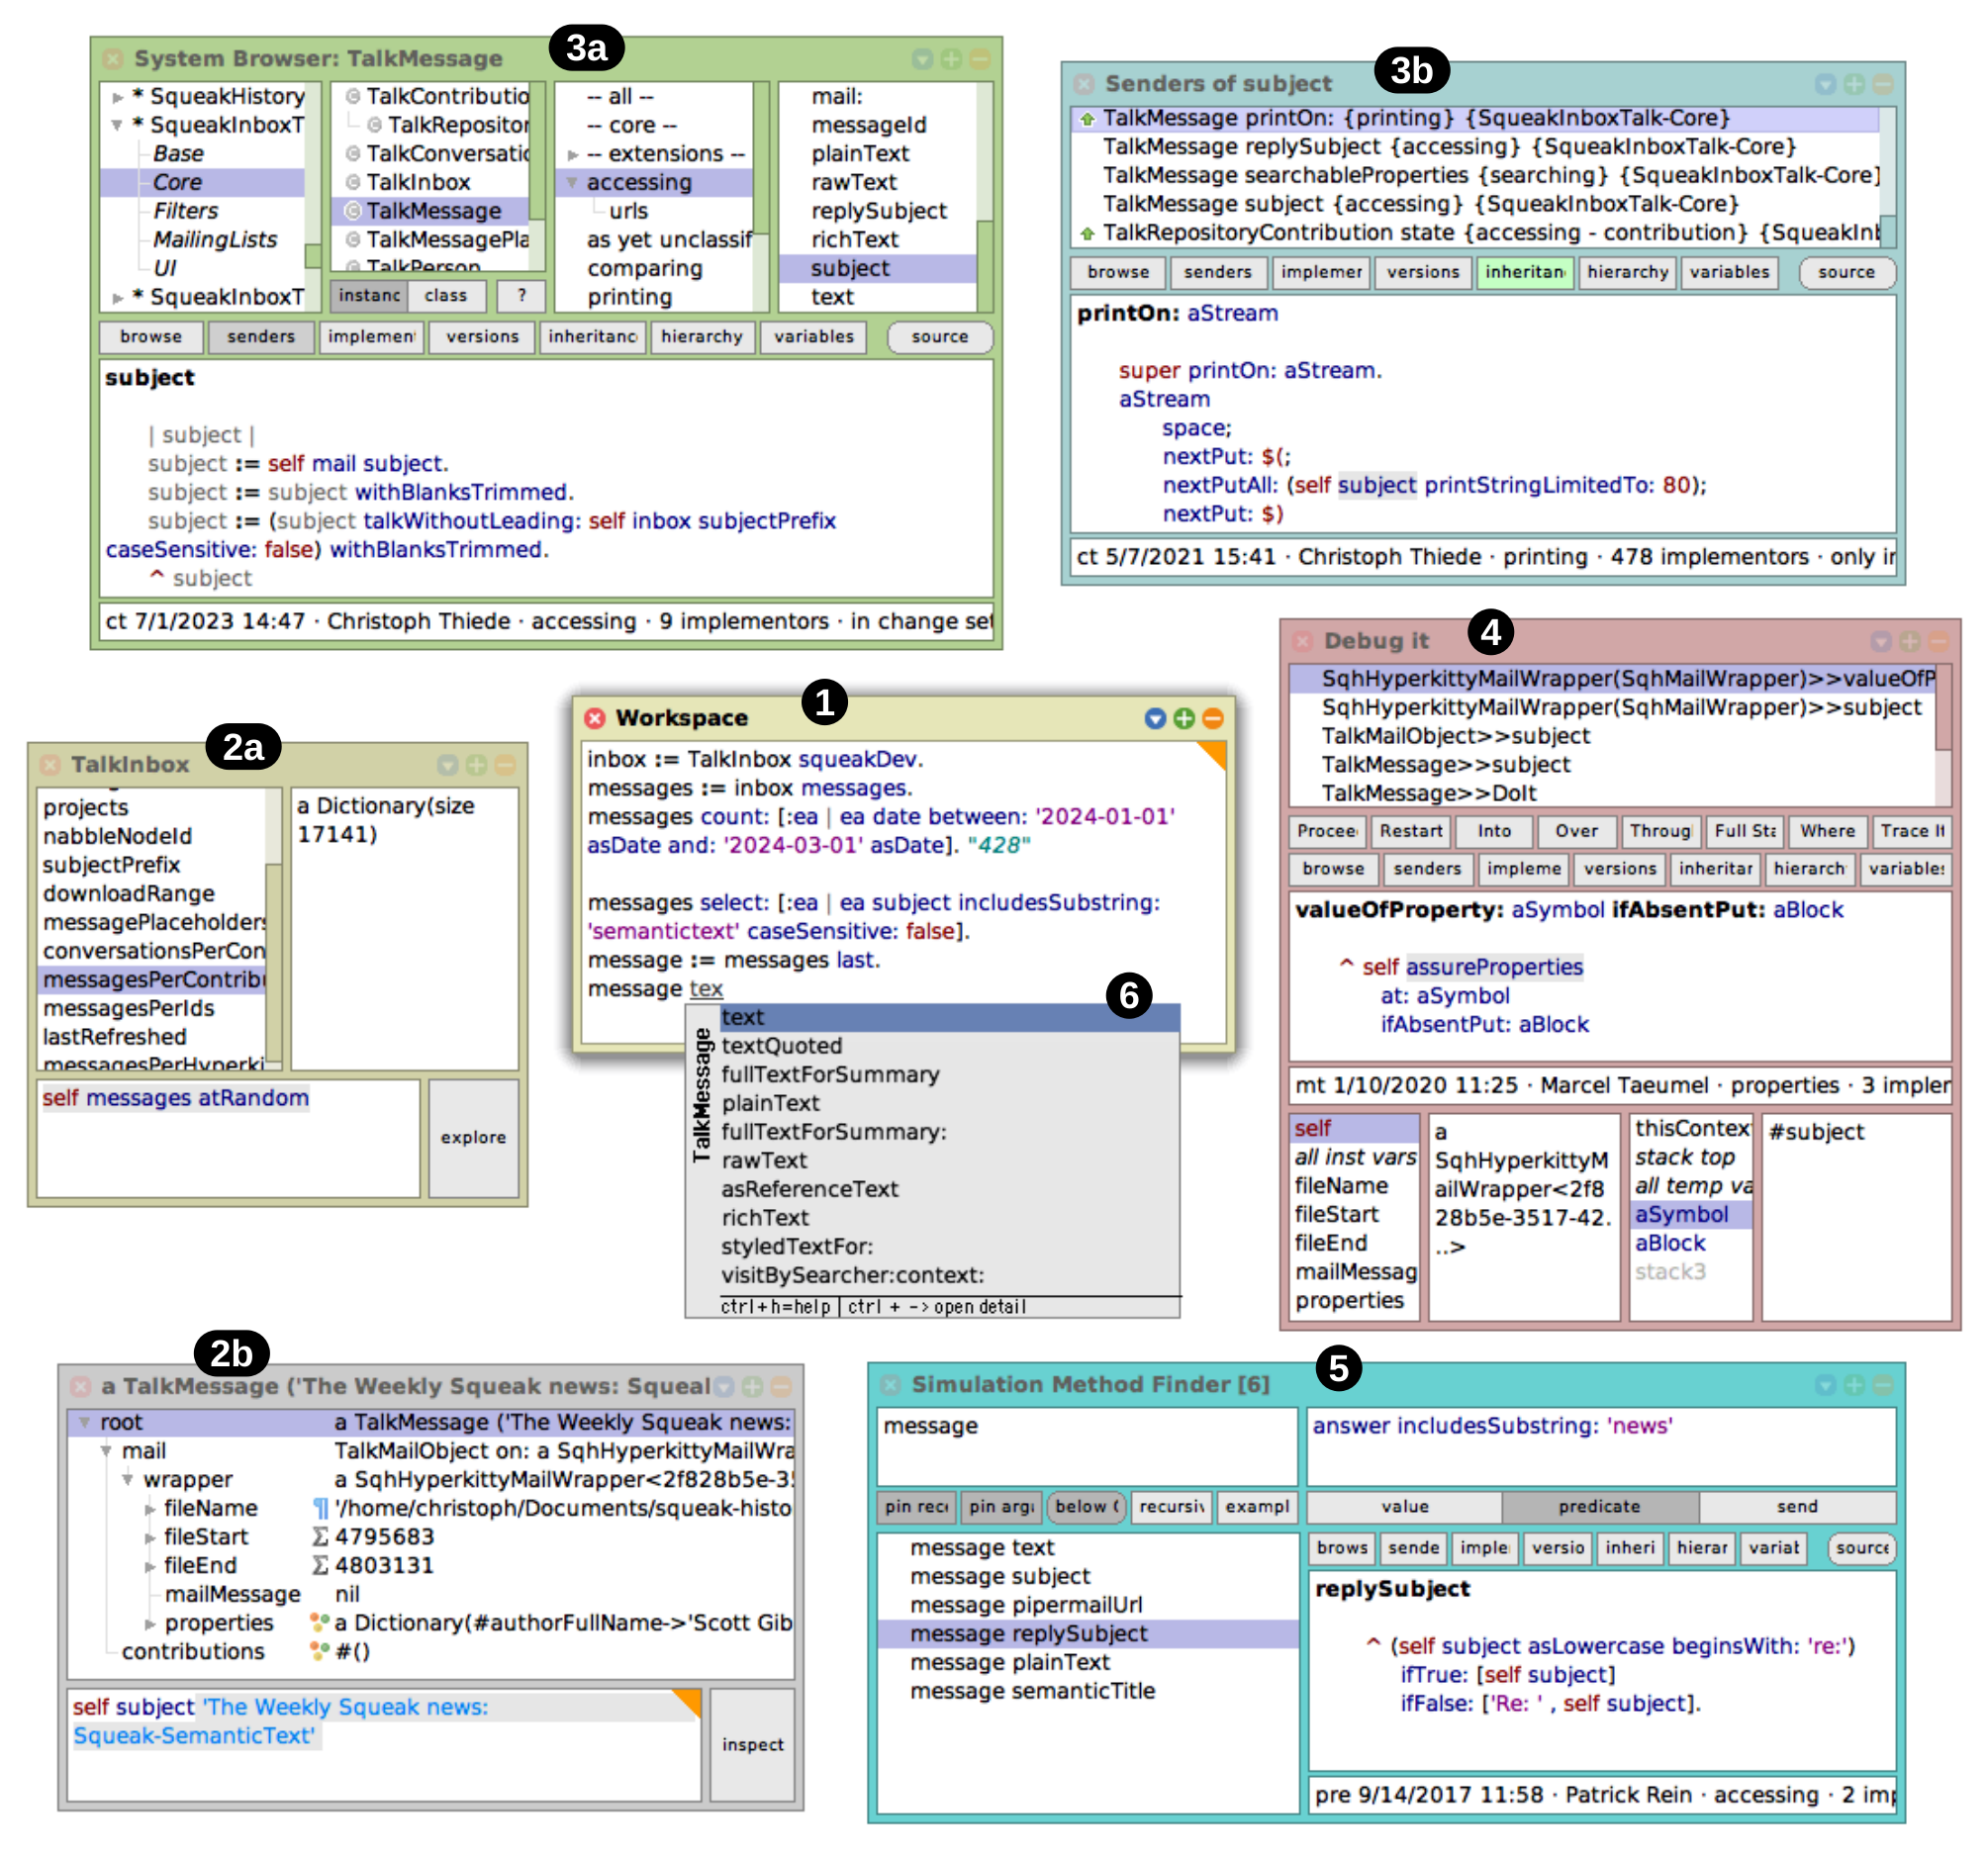
\includegraphics[width=\textwidth]{02_expsys/squeak_tools.png}
		% todo: larger?
		\caption[A collection of \emph{exploratory programming tools} in the Squeak"/Smalltalk system.]{
			A collection of different interconnected tools in the exploratory programming system Squeak"/Smalltalk.
			At the heart is the workspace \Circled{1} through which programmers can execute \emph{do-it} code snippets to retrieve information from objects.
			From the workspace, programmers can invoke other tools such as \emph{object inspection tools} to examine the variables (\Circled{2a} inspector) and nested properties (\Circled{2b} explorer) of particular objects, \emph{code browsing tools} to study the implementation of methods (\Circled{3a} system browser) or their users (\Circled{3b} message trace), \emph{debugging tools} to explore method behavior in context (\Circled{4} debugger), \emph{symbolic execution tools} to find messages through constraints (\Circled{5} simulation method finder\footnote{\url{https://github.com/LinqLover/SimulationStudio}}), or \emph{code completion tools} to browse available protocols in an editor context (\Circled{6} Autocompletion\footnote{\url{https://github.com/LeonMatthes/Autocompletion}}).
			Each of these tools can assist programmers in different parts of their exploratory process by providing domain- or task-specific support.
		}
		\label{fig:background/expsys/squeak_tools}
	\end{minipage}
\end{figure}

%\begin{description}
%	\item[Object inspection tools]
	\paragraph{Object inspection tools}
	\label{par:background/expsys/tools/inspection}
	Through inspection tools, programmers can explore and modify the internal state of any object in the system.
	The standard inspection tools in Squeak are the \emph{inspector} and \emph{explorer}, which provide low-level access to the list of instance variables or fields in an object~\cites[chap.~8]{goldberg1984smalltalk}[sec.~6.3]{thiede2023squeak}.

	However, inspection tools can also provide higher-level, domain-specific interfaces to objects:
	for example, \emph{collection inspectors} display and manipulate the effective elements of different types of collection objects independently of their internal data structure; other systems such as \name{Glamorous Toolkit}'s \emph{moldable inspector} promote domain-specific visualizations of objects such as charts or graphs~\cite{chis2015moldable}.
	Thus, programmers can directly find answers to more conceptual questions such as ``How are these nodes connected?'' without writing technical do-it scripts on their own.

	%\item[Code browsing tools]
	\paragraph{Code browsing tools}
	\label{par:background/expsys/tools/browsing}
	Through browsing tools, programmers can explore and modify the implementation, protocols, and documentation of classes~\cite[sec.~6.2]{thiede2023squeak}.
	In Squeak, different code browsers allow programmers to navigate and search software systems along their organization and inner relationships:
	\emph{system browsers} provide access to classes through package structures or class hierarchies~\cite[chap.~9]{goldberg1984smalltalk}; \emph{message traces} and similar tools can be used to explore methods through different usage graphs~\cite[chap.~10]{goldberg1984smalltalk}.
	For example, the \emph{senders"/implementors} mechanism allows programmers to browse an (approximate\footnotemark) static call graph of methods that send or implement a given message name~\cite{thiede2022augmenting}; other types of graph queries include references and assignments to variables, methods that contain certain literals (constants), or a full-text search through source code and comments.
	\footnotetext{%
		\label{fn:dynamic_dispatching}
		Messages in Smalltalk are dispatched dynamically, and traditional Smalltalk systems do not have a typing system, preventing them from accurately predicting which methods a message send in a code snippet might activate.
	}

	Thus, code browsing tools provide means for programmers to answer questions about the organization and implementation of systems through high-level and task-specific views and query interfaces.

	%\item[Debugging tools]
	\paragraph{Debugging tools}
	\label{par:background/expsys/tools/debugging}
	In the first place, (symbolic) debuggers were designed to allow programmers to examine faulty programs by executing them step-by-step and finding the underlying cause of a bug~\cites[sec.~17.4]{goldberg1983smalltalk}[sec.~18f.]{goldberg1984smalltalk}.
	However, debuggers have also proven as useful tools for exploring the behavior of software systems beyond bug-fixing, as they provide a concrete context for comprehending abstract source code and navigating through an actual call graph of a program~\cite[sec.~6.4]{thiede2023squeak}.
	Many tools also support \emph{programming in the debugger} to modify the behavior of a running program, which allows for a ``programming into existence'' practice for interface-first, iterative prototyping~\cite{rosson1993active}.
	\emph{Babylonian programming} environments promote a similar practice by integrating the execution context of different examples into regular code browsing tools~\cite{rauch2019babylonian}.

	\emph{Back-in-time debuggers} (also referred to as \emph{time-travel debuggers} or \emph{omniscient debuggers}) record the execution of a program or re-run it repeatedly to allow programmers to explore it independently of the original execution order~\cite{lewis2003debugging,pothier2009back,perscheid2014follow}.
	On top of such an omniscient perspective on programs, they offer different interfaces for navigating programs along objects, dataflows~\cite{lienhard2009taking}, or state changes~\cite{thiede2023object,thiede2023time} or for visualizing the program execution~\cite{thiede2024bringing}. % cornelissen2008execution
	For example, the \name{Whyline} approach provides a query interface where programmers can combine prepared natural-language blocks to ask a range of questions about the causes of certain events in a program~\cite{ko2004designing}.

	% todo: just another summary here?

	%\item[Symbolic execution tools]
	\paragraph{Symbolic execution tools}
	\label{par:background/expsys/tools/symbex}
	\emph{Symbolic execution engines} make it possible to execute programs and send messages to objects despite the lack of concrete context by substituting unknown state with symbols and executing all possible code paths concurrently~\cite{cadar2013symbolic,thiede2023symbolic}.
	This provides a basis for exploratory programming tools that can search the behavior of objects through speculative execution.
	Squeak's \emph{method finder} allows programmers to find unknown methods by specifying constraints over the inputs and outputs of message sends~\cite[sec.~1.8]{thiede2023squeak}%
	\footnote{While Squeak does not include a symbolic execution engine at the time of writing, the method finder employs equivalent brute-force strategies to resolve the provided constraints.}%
	\footnote{
		An evolved version of Squeak's built-in method finder is available through the \name{SimulationStudio} package.
		Christoph Thiede: ``Method Finder 2.'' The general-purpose Squeak developers list, 2022-09-20. URL:
		%\url{https://lists.squeakfoundation.org/archives/list/squeak-dev@lists.squeakfoundation.org/thread/N4OM3BYARXMOFDF4ONM7IZWR7727WU2M}.
		\url{https://web.archive.org/web/20240630205751/https://lists.squeakfoundation.org/archives/list/squeak-dev@lists.squeakfoundation.org/thread/N4OM3BYARXMOFDF4ONM7IZWR7727WU2M/}
	}%
	.
	Tools such as \name{IntelliTest}\footnote{
		%\url{https://learn.microsoft.com/en-us/visualstudio/test/intellitest-manual}
		\url{https://web.archive.org/web/20240530170603/https://learn.microsoft.com/en-us/visualstudio/test/intellitest-manual/?view=vs-2022}
	} or \name{SED}~\cite{hentschel2019symbolic} provide programmers with an overview of different code paths and examples for methods.

	Thus, symbolic execution tools allow programmers to research the methods of objects by asking questions about their effective behavior without browsing or manually executing them.

	%\item[Code completion tools]
	\paragraph{Code completion tools}
	\label{par:background/expsys/tools/completion}
	Autocompletion tools support programmers at writing code by automatically suggesting possibly relevant message names (also referred to as \emph{selectors}) and variables next to the text caret.
	Suggestions can be contextualized in various degrees, e.g., by considering the syntactic context of existing code, usage statistics from the current programming session~\cite{robbes2008program}, or information from runtime or typing systems~\cite{pluquet2009fast}.
	Some modern code completion tools also employ large language models to suggest completions of entire statements or methods~(see \cref{sec:background/semtec}).

	Beside accelerating typing, code completion tools also support the research process of exploratory programmers by providing them with possible answers to questions about the usage of protocols (``What messages can I send to this variable?'') and making manual research through code browsing tools superfluous in some cases.
%\end{description}

\ParSep

By using and combining different kinds of tools offered by exploratory programming systems, programmers can derive more informed answers to questions and delegate low-level parts of their research process to the system.

% todo: screenshots?
